\section{Профиль и протокол}
\subsection{Цель и модели}
Цель --- сравнить энергетическое и обратимое представления распределения при общих данных и близкой ёмкости~\cite{teacher}. EBM задаёт $p_\theta(x)=e^{-E_\theta(x)}/Z_\theta$. Использована энергия
\begin{equation}E_\theta(x)=\|x\|^2/(2s^2)+r_\theta(x),\qquad s=3,\quad r_\theta=\tanh(\operatorname{MLP}_\theta(x)).\end{equation}
Ограниченный остаток обеспечивает конечность $Z_\theta$. Сеть E1 имеет три скрытых слоя ширины 128 с ReLU. Отрицательная фаза обучается на отсоединённых входах $x^-$: loss $\overline{E(x^+)}-\overline{E(x^-)}$. Градиент по параметрам энергии сохраняется; через саму цепь он не проводится.

Сэмплер без поправки Метрополиса использует
\begin{equation}x_{k+1}=x_k-\eta\nabla_xE(x_k)+\sqrt{2\eta T}\,\epsilon_k,\quad T=1.\end{equation}
Основной режим отражает точки в $\Omega=[-15,15]^2$. Replay имеет ёмкость 10 000, случайное вытеснение и вероятность нового нормального старта 0.05. Всегда $K=50$; короткая цепь не объявляется точной выборкой стационарного EBM.

Flow преобразует данные в стандартный нормальный шум $z=f(x)$:
\begin{equation}\log p_X(x)=\log p_Z(f(x))+\log|\det J_f(x)|.\end{equation}
Аффинный coupling оставляет $x_a$ и преобразует $x_b$: $y_b=x_b\exp(s_\theta(x_a))+t_\theta(x_a)$. Логарифм определителя равен сумме $s_\theta$, обратный шаг явный. Сети $s,t$ имеют по два скрытых слоя ширины 64; $s_\theta=c\tanh(\tilde s_\theta/c)$, $c=4$. Между coupling меняются координаты. Обратный проход идёт в обратном порядке.

\subsection{Данные и оценка}
Профиль: трудная цель eight gaussians, шаги 0.005,0.02,0.08,0.5, $c=4$. E1/E2 используют two blobs: центры $(\pm2,0)$, $\sigma=0.3$. E3 использует восемь равновероятных компонент с центрами $3(\cos(2\pi m/8),\sin(2\pi m/8))$, $\sigma=0.2$. Для каждой цели train/val/test = 20 000/5000/5000, seeds 601/602/603. Координаты не стандартизованы, cal не создаётся. Формальные модели: CPU, два потока, float32, Adam 0.001, batch 256, ровно 5000 обновлений.

Для качества генерируется 5000 точек. Ближайшая мода назначается в радиусе $3\sigma$, остальные точки образуют внешнюю категорию. $Cov$ --- доля мод с частотой не ниже половины истинного веса; $D_{mode}$ --- половина суммы абсолютных разностей частот модели и фиксированного test, включая внешнюю категорию. MMD$^2$ --- V-статистика с RBF-ядром. Ширина ядра фиксирована для цели по медиане расстояний на 2000 train-точках, seed 604; шум оценён пятью свежими выборками цели.

EBM нормируется только на сетке $120\times120$ центров ячеек, шаг 0.25, площадь 0.0625. Его $\hat p_\Omega$ и $D_{grid}$ --- приближённые величины; точный NLL вычисляется только для Flow. Ошибка обратимости $\varepsilon_{inv}=\|x-f^{-1}(f(x))\|/(\|x\|+10^{-8})$ проверяется отдельно от якобиана.

\section{E1. Шаг Ланжевена}
Одна EBM обучена на two blobs и заморожена (R20). Энергия обоих центров $-0.777778$, в нуле 1, средняя test-энергия $-0.717557$. Центры ниже промежутка. Верхняя граница ненормированного хвостового интеграла вне радиуса 14 равна $e\,2\pi9\exp(-14^2/18)=0.002869$, меньше 0.01; это не точная хвостовая вероятность.
\begin{figure}[H]\centering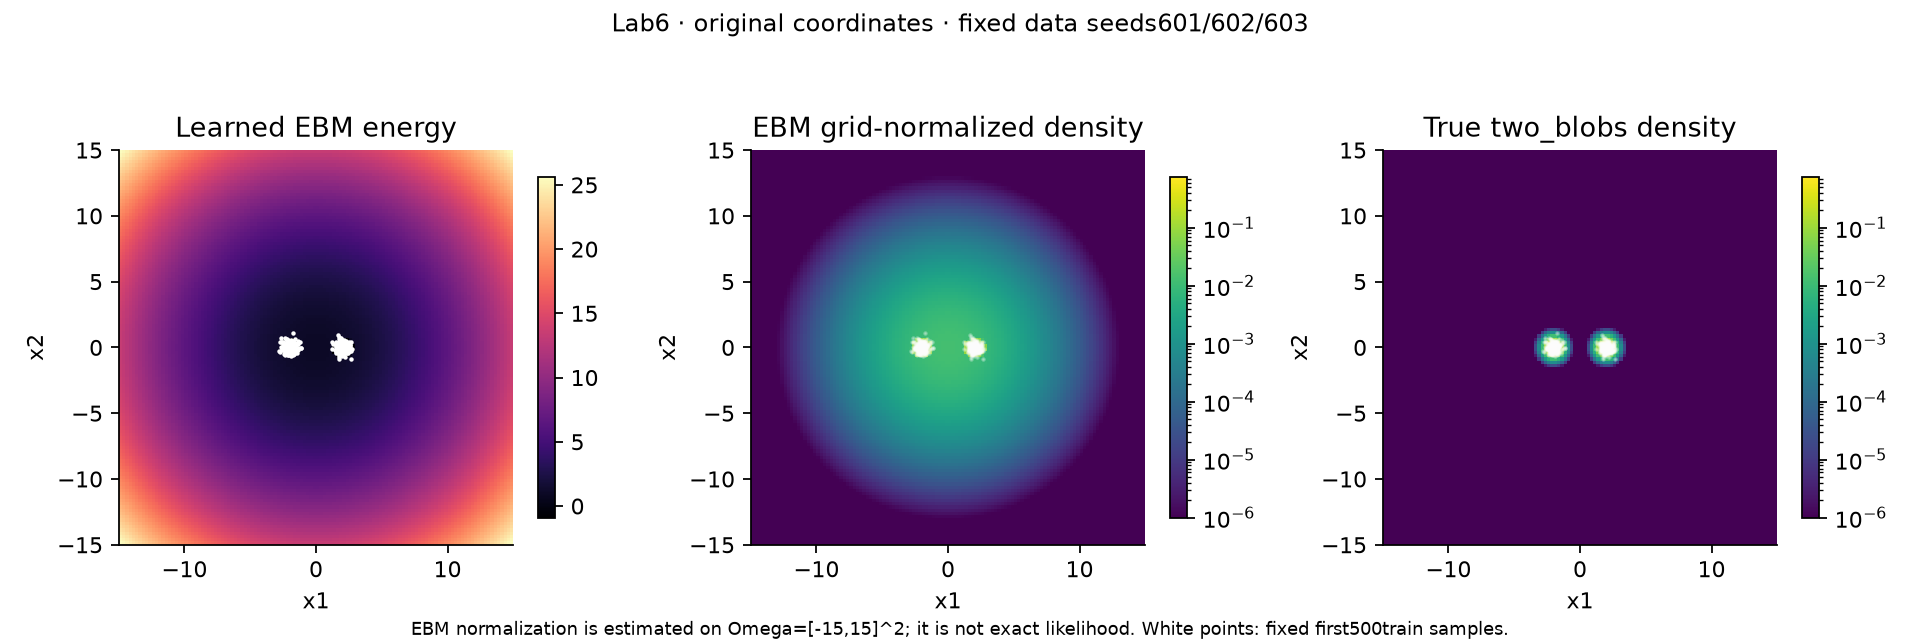
\includegraphics[width=\linewidth,height=.37\textheight,keepaspectratio]{figures/density.png}
\caption{E1: энергия, нормированная на квадрат сеточная плотность и данные two blobs.}\label{fig:density}
\end{figure}

\begin{table}[H]\centering\small
\setlength{\tabcolsep}{4pt}
\caption{E1: один обученный EBM, четыре шага сэмплера, $K=50$.}\label{tab:eta}
\begin{tabular}{rrrrrrl}
\toprule
$\eta$ & MMD$^2$ & Cov & $D_{mode}$ & $D_K$ & Смена моды & Ист. \\
\midrule
0.005 & 0.052331 & 0.0 & 0.7476 & 0.8926 & 0.00\% & R01 \\
0.02 & 0.037175 & 0.0 & 0.7582 & 1.7286 & 0.70\% & R02 \\
0.08 & 0.129107 & 0.0 & 0.9150 & 3.2972 & 1.78\% & R03 \\
0.5 & 0.203648 & 0.0 & 0.9320 & 4.5117 & 2.92\% & R04 \\
\bottomrule
\end{tabular}
\end{table}


\begin{figure}[H]\centering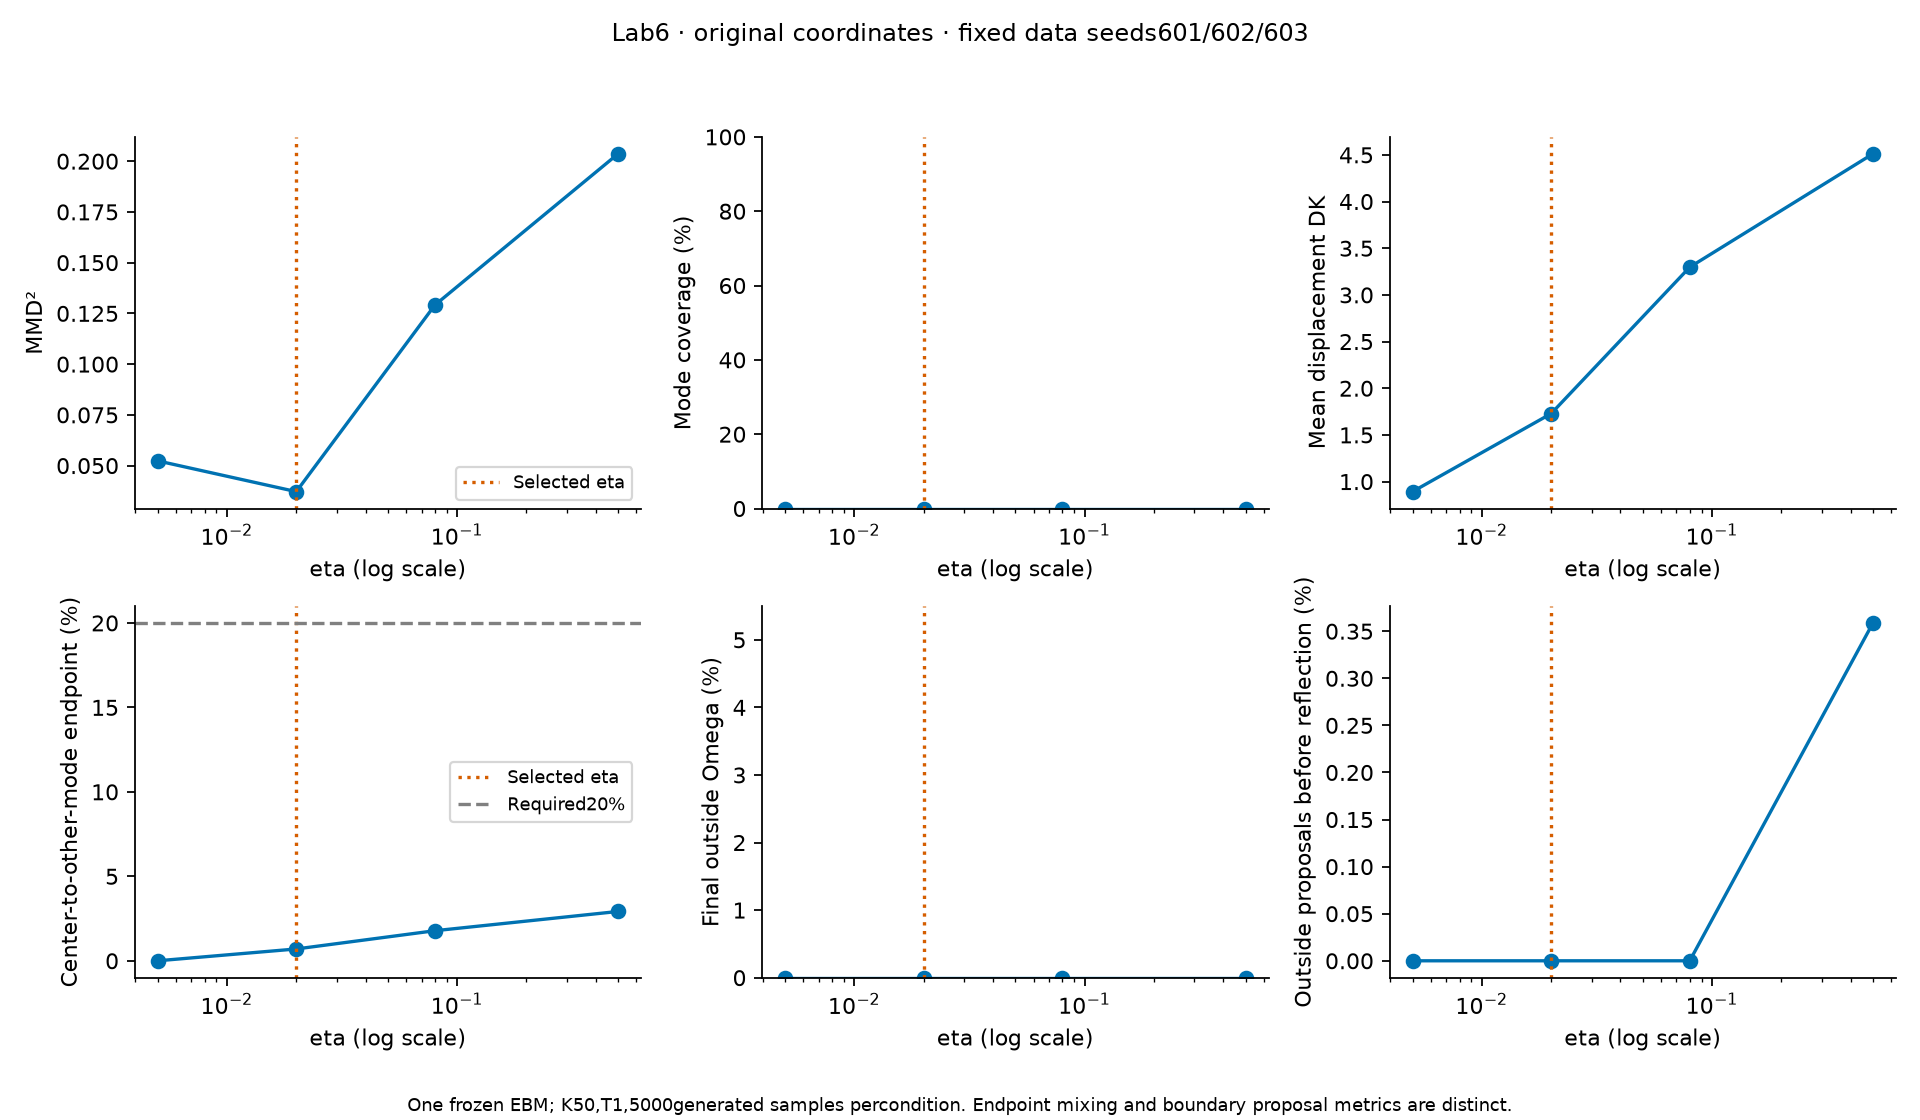
\includegraphics[width=\linewidth,height=.38\textheight,keepaspectratio]{figures/etafig.png}
\caption{E1: качество и смещение короткой цепи при изменении шага.}\label{fig:etafig}
\end{figure}

Все цепи численно устойчивы и после отражения остаются в области. Доля выходящих предложений до отражения достигает 0.3588\% при 0.5. Ни один шаг не обеспечил 20\% переходов из одного центра к другой моде: максимум 2.92\%. Первичный критерий смешивания не выполнен. По предусмотренному заданием резервному правилу выбран устойчивый шаг с минимальной MMD$^2$, $\eta=0.02$. Наименьший шаг даёт малое смещение, наибольший --- наибольший дискретизационный сдвиг квадратичной цепи и худшую MMD. Нулевой Cov во всех четырёх условиях сохраняется как отрицательный результат.
\begin{figure}[H]\centering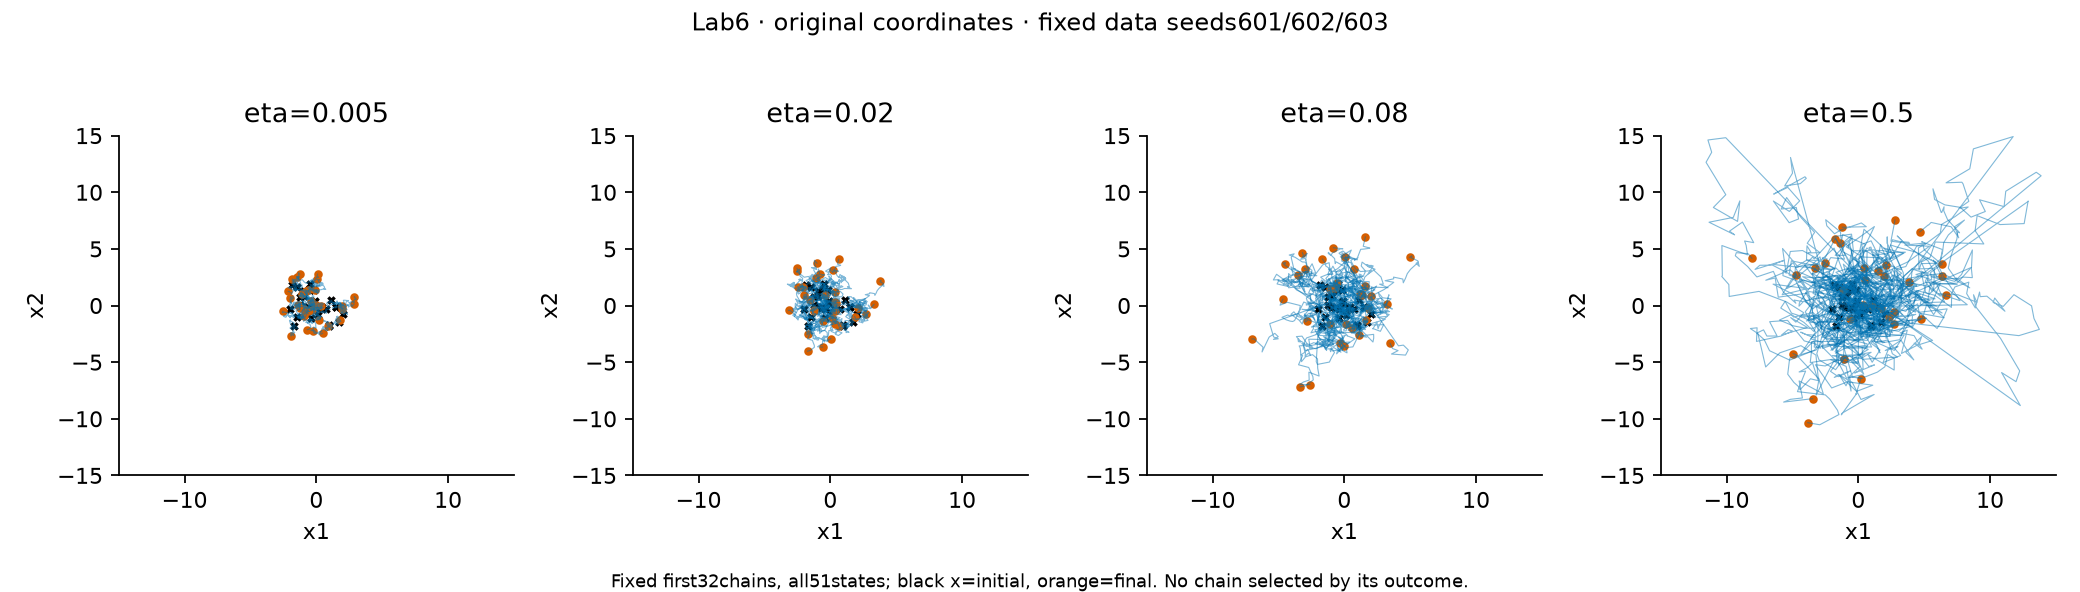
\includegraphics[width=\linewidth,height=.35\textheight,keepaspectratio]{figures/trajectories.png}
\caption{Сохранённые траектории одной замороженной энергии.}\label{fig:trajectories}
\end{figure}

Для $E(x)=x^2/2$ без границ рекурсия AR(1) имеет стационарную дисперсию
\begin{equation}v=\frac{\sigma^2}{2\eta-\eta^2},\qquad \sigma^2=2\eta\ \Rightarrow\ v=\frac1{1-\eta/2}.\end{equation}
Каждая проверка содержит восемь независимых цепей, 10 000 burn-in и 200 000 сохранённых шагов на цепь. Это реально исполненные конечные рекурсии, не аналитическая генерация стационарных точек.
\begin{table}[H]\centering\small
\setlength{\tabcolsep}{4pt}
\caption{Дисперсия длинной безграничной квадратичной цепи; последняя строка --- контроль с неверным шумом.}\label{tab:quadratic}
\begin{tabular}{rrrrrrl}
\toprule
$\eta$ & $\sigma$ & $T_{eff}$ & $v_{theory}$ & $v_{measured}$ & Отн. ошибка & Ист. \\
\midrule
0.005 & 0.1 & 1.00 & 1.0025063 & 1.0056753 & 0.316\% & R05 \\
0.02 & 0.2 & 1.00 & 1.0101010 & 1.0011181 & 0.889\% & R06 \\
0.08 & 0.4 & 1.00 & 1.0416667 & 1.0443116 & 0.254\% & R07 \\
0.5 & 1.0 & 1.00 & 1.3333333 & 1.3343135 & 0.074\% & R08 \\
0.5 & 0.2 & 0.04 & 0.0533333 & 0.0534600 & 0.238\% & R09 \\
\bottomrule
\end{tabular}
\end{table}


\begin{figure}[H]\centering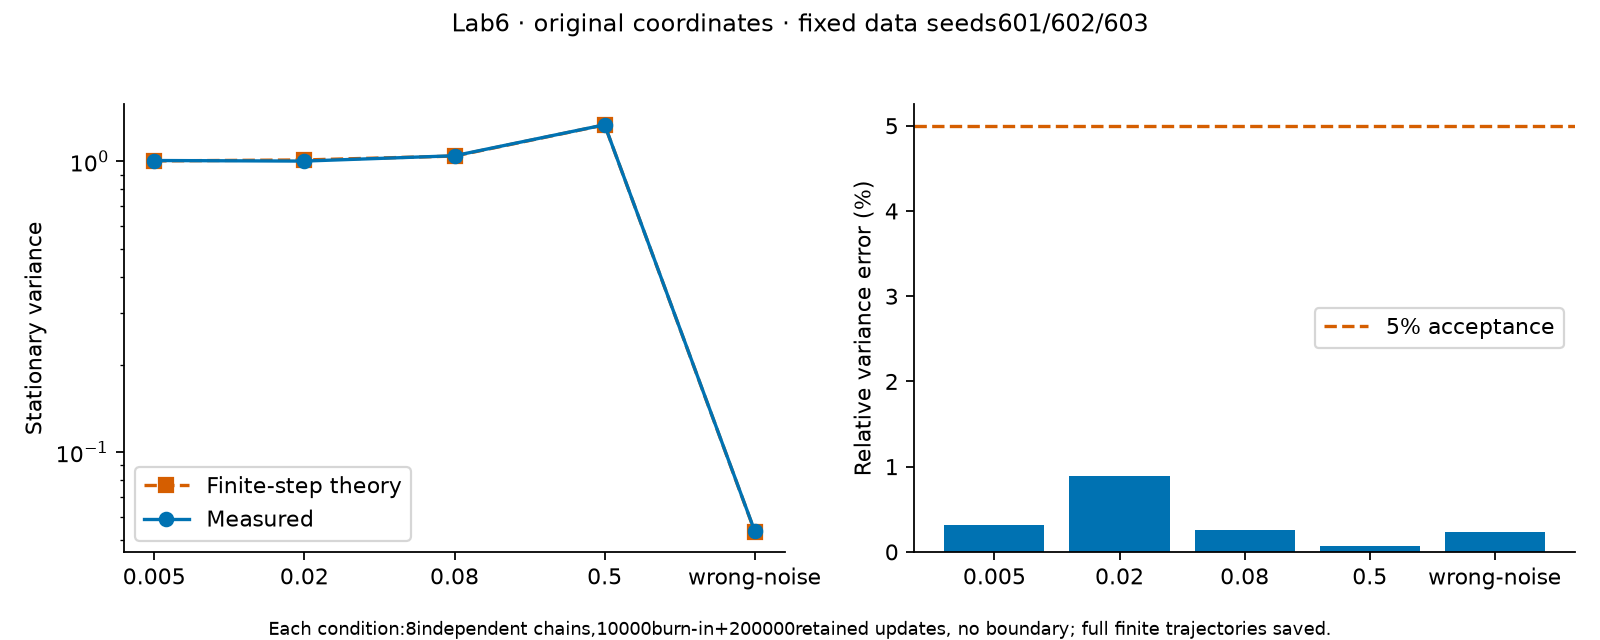
\includegraphics[width=\linewidth,height=.31\textheight,keepaspectratio]{figures/quadfig.png}
\caption{Предсказанная и измеренная дисперсия; неверный шум показан отдельно.}\label{fig:quadfig}
\end{figure}

Ошибки всех дисперсий меньше 5\%. У выученной энергии ограниченный tanh допускает разность остатка не больше 2, а квадратичный prior масштаба 3 намного шире облаков масштаба 0.3. Низкая энергия центров не обеспечивает концентрацию плотности возле них и достаточное смешивание за 50 шагов.

\section{E2. Глубина потока}
При одинаковых seed, бюджете и оптимизации меняется только $K_f$. Правдоподобие выбирается по val; test не участвует в выборе глубины.
\begin{table}[H]\centering\scriptsize
\setlength{\tabcolsep}{4pt}
\caption{E2: все глубины потока и медианная ошибка обратимости в float64.}\label{tab:depth}
\begin{tabular}{rrrrrrrrl}
\toprule
$K_f$ & Val NLL & SEM & MMD$^2$ & Cov & Параметры & $\varepsilon_{test}$ & $\varepsilon_{20}$ & Ист. \\
\midrule
2 & 2.34482 & 0.01056 & 0.0129 & 0.0 & 17412 & 1.38e-17 & 4.44e-17 & R10 \\
4 & 1.17997 & 0.01532 & 0.000226 & 1.0 & 34824 & 1.16e-16 & 1.36e-13 & R11 \\
8 & 1.13468 & 0.01465 & 9.68e-05 & 1.0 & 69648 & 1.27e-16 & 3.69e-13 & R12 \\
16 & 1.13971 & 0.01386 & 7.43e-05 & 1.0 & 139296 & 1.59e-16 & 3.03e-07 & R13 \\
\bottomrule
\end{tabular}
\end{table}


\begin{figure}[H]\centering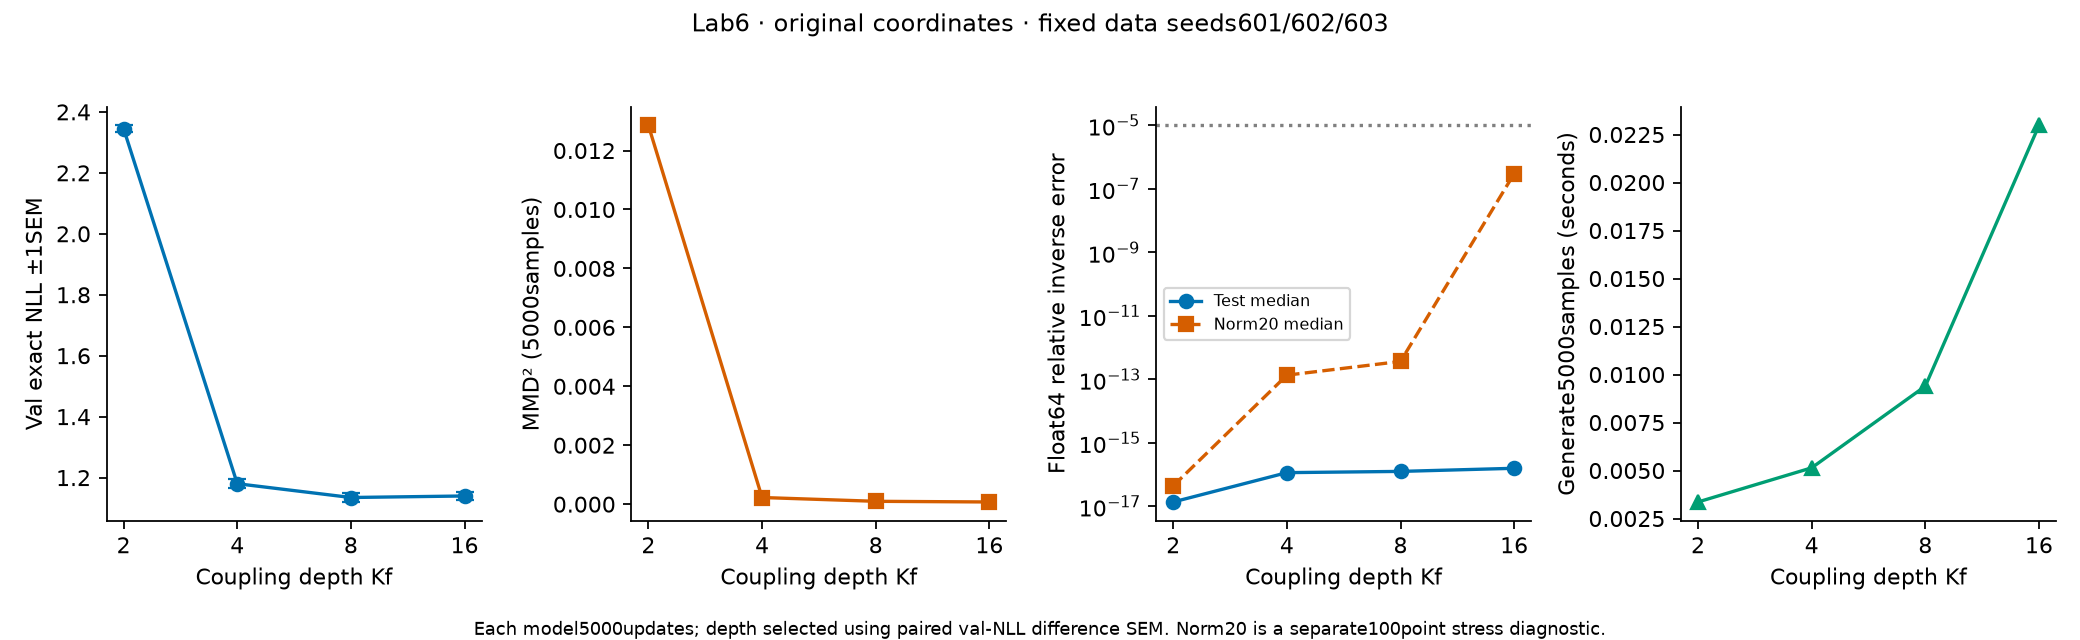
\includegraphics[width=\linewidth,height=.41\textheight,keepaspectratio]{figures/depthfig.png}
\caption{E2: правдоподобие, качество и обратимость при изменении глубины.}\label{fig:depthfig}
\end{figure}

Выигрыши val NLL при 2$\to$4, 4$\to$8, 8$\to$16 равны 1.164845, 0.045297, $-0.005034$; SEM парных разностей на тех же val-точках --- 0.010758,0.004523,0.002966. Первые два улучшения превышают две SEM, третье --- нет. Выбрана минимальная глубина перед незаметным следующим улучшением: $K_f=8$.

Медианные ошибки на test значительно меньше $10^{-5}$; максимальное расхождение logdet с autograd не превосходит $4.31\cdot10^{-14}$. Для этой диагностики сохранённые обученные веса переведены в float64, обучение не повторялось. На норме 20 ошибка растёт: для 16 слоёв медиана $3.03\cdot10^{-7}$, максимум $1.07\cdot10^{-4}$. Порог для области данных не переносится на стресс-точки; эта численная граница не меняет выбранные $c$ и глубину.

\section{E3. EBM и Flow на трудной цели}
До запусков сформулирована гипотеза: $\Delta_s=\mathrm{MMD}^2_{EBM,s}-\mathrm{MMD}^2_{Flow,s}>0$, поскольку короткие цепи могут плохо достигать узких разнесённых мод. Неустойчивый знак или отсутствие установленного положительного эффекта опровергли бы прогноз. Фиксированы цель, данные, область, 5000 обновлений, batch, Adam, три общих seed, $\eta=0.02$, $K=50$, $K_f=8$, $c=4$. Меняется класс модели; для выравнивания ёмкости ширина EBM 185: 69 561 параметр против 69 648 у Flow, разница 0.1251\%.
\begin{table}[H]\centering\footnotesize
\setlength{\tabcolsep}{4pt}
\caption{E3: 5000 генерируемых точек на каждый seed и модель.}\label{tab:models}
\begin{tabular}{llrrrrrl}
\toprule
Seed & Модель & Cov & $D_{mode}$ & MMD$^2$ & Train, с & Sample, с & Ист. \\
\midrule
1 & EBM & 0.0 & 0.8382 & 0.01290224 & 379.78 & 0.88385 & R14 \\
1 & FLOW & 1.0 & 0.0858 & 0.00015828 & 84.47 & 0.00909 & R15 \\
2 & EBM & 0.0 & 0.8402 & 0.01245476 & 352.65 & 0.83343 & R16 \\
2 & FLOW & 1.0 & 0.1012 & 0.00028826 & 79.51 & 0.01138 & R17 \\
3 & EBM & 0.0 & 0.8514 & 0.01486872 & 347.57 & 0.72787 & R18 \\
3 & FLOW & 1.0 & 0.0978 & 0.00027719 & 79.31 & 0.00983 & R19 \\
\bottomrule
\end{tabular}
\end{table}


\begin{table}[H]\centering\small
\setlength{\tabcolsep}{4pt}
\caption{Разные характеристики плотности; NLL Flow точен, $D_{grid}$ EBM нормирован на $\Omega$.}\label{tab:density}
\begin{tabular}{rrrrl}
\toprule
Seed & Flow test NLL & EBM $D_{grid}$ & $\hat Z_\Omega$ & Ист. EBM/Flow \\
\midrule
1 & 2.037256 & 0.0014933 & 31.8476 & R14/R15 \\
2 & 2.039678 & 0.0015173 & 32.5688 & R16/R17 \\
3 & 2.031565 & 0.0015976 & 29.9522 & R18/R19 \\
\bottomrule
\end{tabular}
\end{table}


\begin{figure}[H]\centering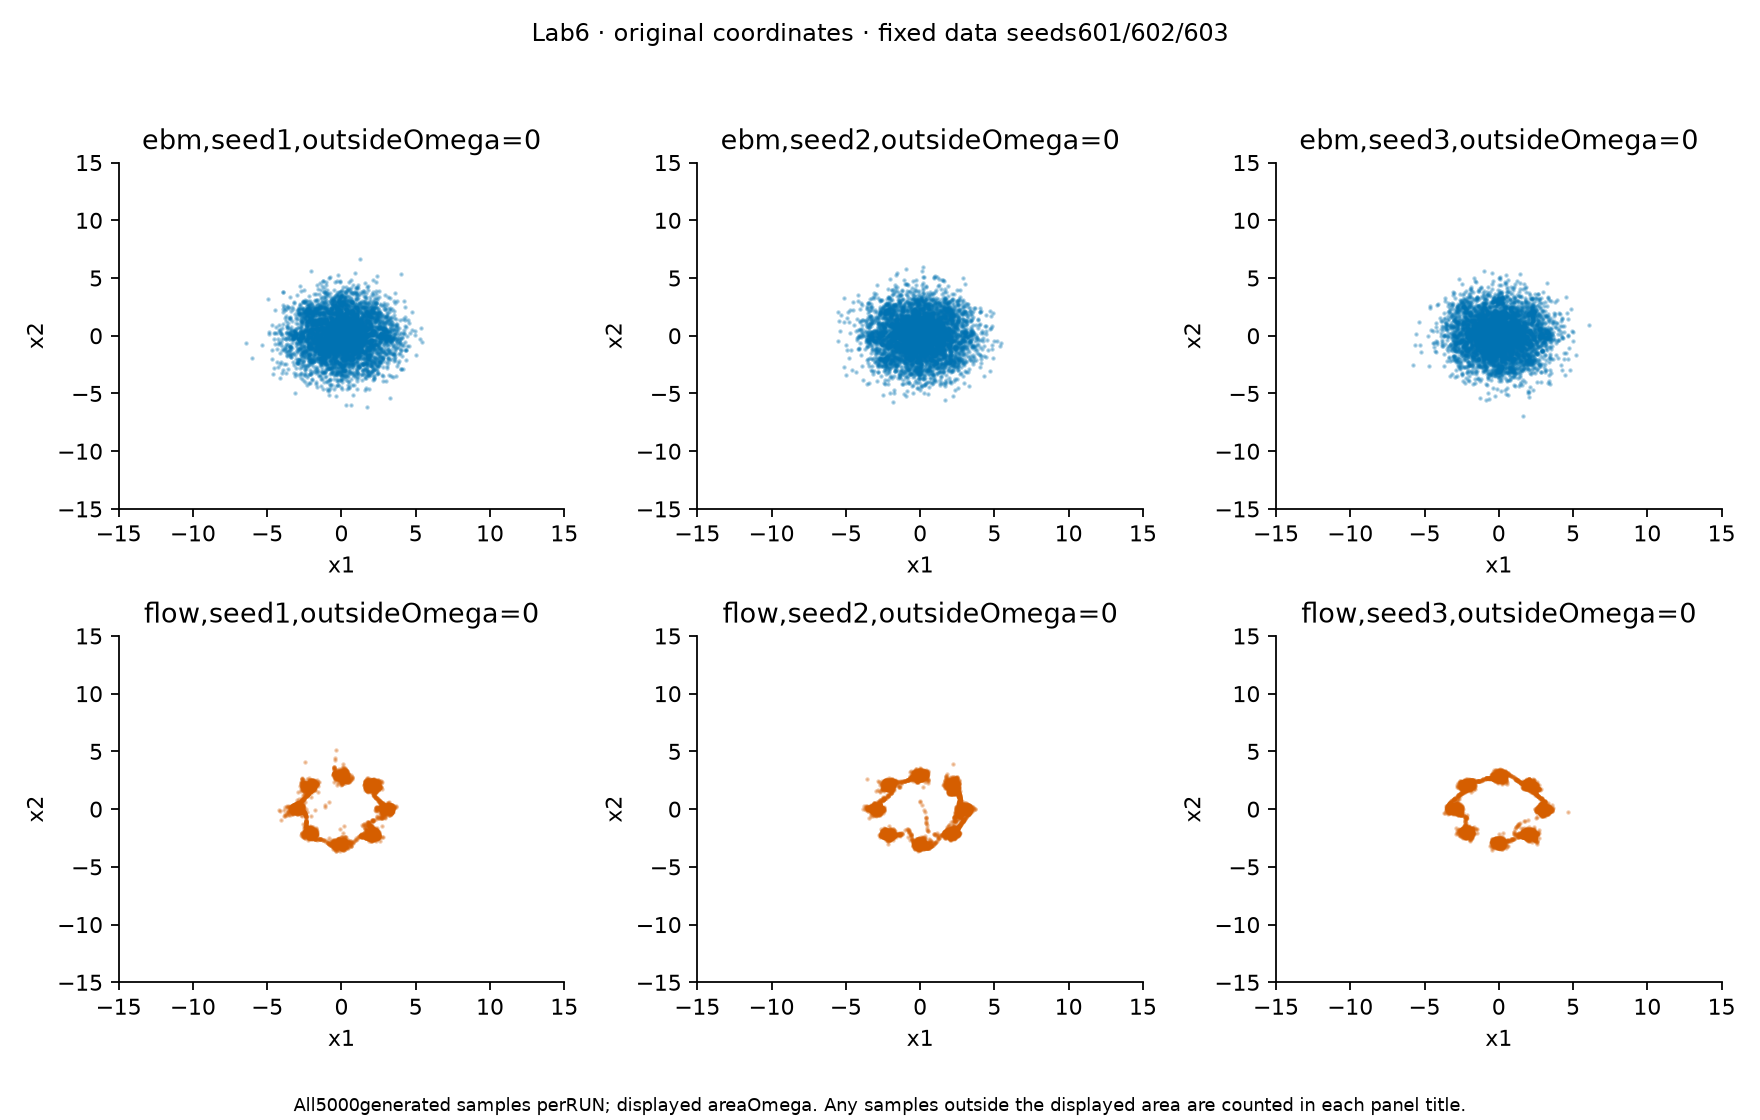
\includegraphics[width=\linewidth,height=.44\textheight,keepaspectratio]{figures/samples.png}
\caption{E3: реальные и порождённые точки для трёх seed.}\label{fig:samples}
\end{figure}

\begin{figure}[H]\centering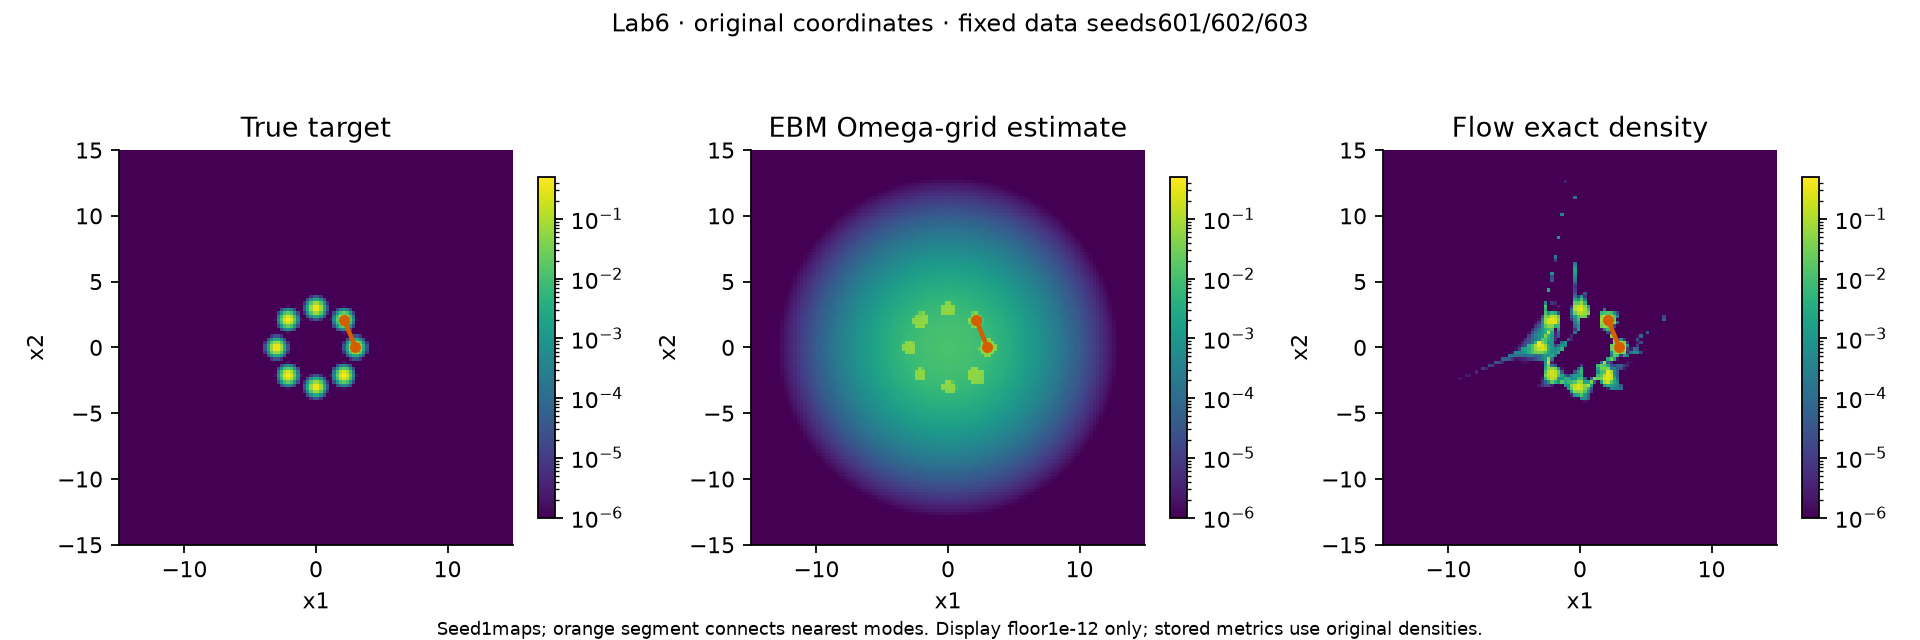
\includegraphics[width=\linewidth,height=.40\textheight,keepaspectratio]{figures/density3.png}
\caption{E3: плотности и промежуток между двумя ближайшими модами.}\label{fig:density3}
\end{figure}

\begin{table}[H]\centering\small
\setlength{\tabcolsep}{4pt}
\caption{Все три парные разности MMD$^2$: EBM минус Flow.}\label{tab:pairs}
\begin{tabular}{rrrr}
\toprule
Seed & EBM & Flow & $\Delta_s$ \\
\midrule
1 & 0.012902242 & 0.000158284 & 0.012743958 \\
2 & 0.012454765 & 0.000288261 & 0.012166504 \\
3 & 0.014868720 & 0.000277187 & 0.014591533 \\
\bottomrule
\end{tabular}
\end{table}


Средняя разность 0.013167332, выборочное SD 0.001266738. Все три знака положительны, среднее больше $2s_\Delta=0.002533476$ и уровня шума MMD$^2=0.000100442$. Различие установлено в пользу Flow; направленная гипотеза поддержана. Это сравнение данных классов с фиксированными генераторами и бюджетом, а не универсальное преимущество обратимых моделей.
\begin{table}[H]\centering\small
\setlength{\tabcolsep}{4pt}
\caption{Логарифмы плотности в середине двух ближайших мод; EBM --- сеточная оценка.}\label{tab:bridge}
\begin{tabular}{rrrrr}
\toprule
Seed & Цель & Flow, точно & EBM, сетка & Flow минус цель \\
\midrule
1 & -16.480539 & -23.625484 & -4.887737 & -7.144945 \\
2 & -16.480539 & -7.298760 & -4.910132 & +9.181779 \\
3 & -16.480539 & -5.690201 & -4.826334 & +10.790338 \\
\bottomrule
\end{tabular}
\end{table}


\begin{figure}[H]\centering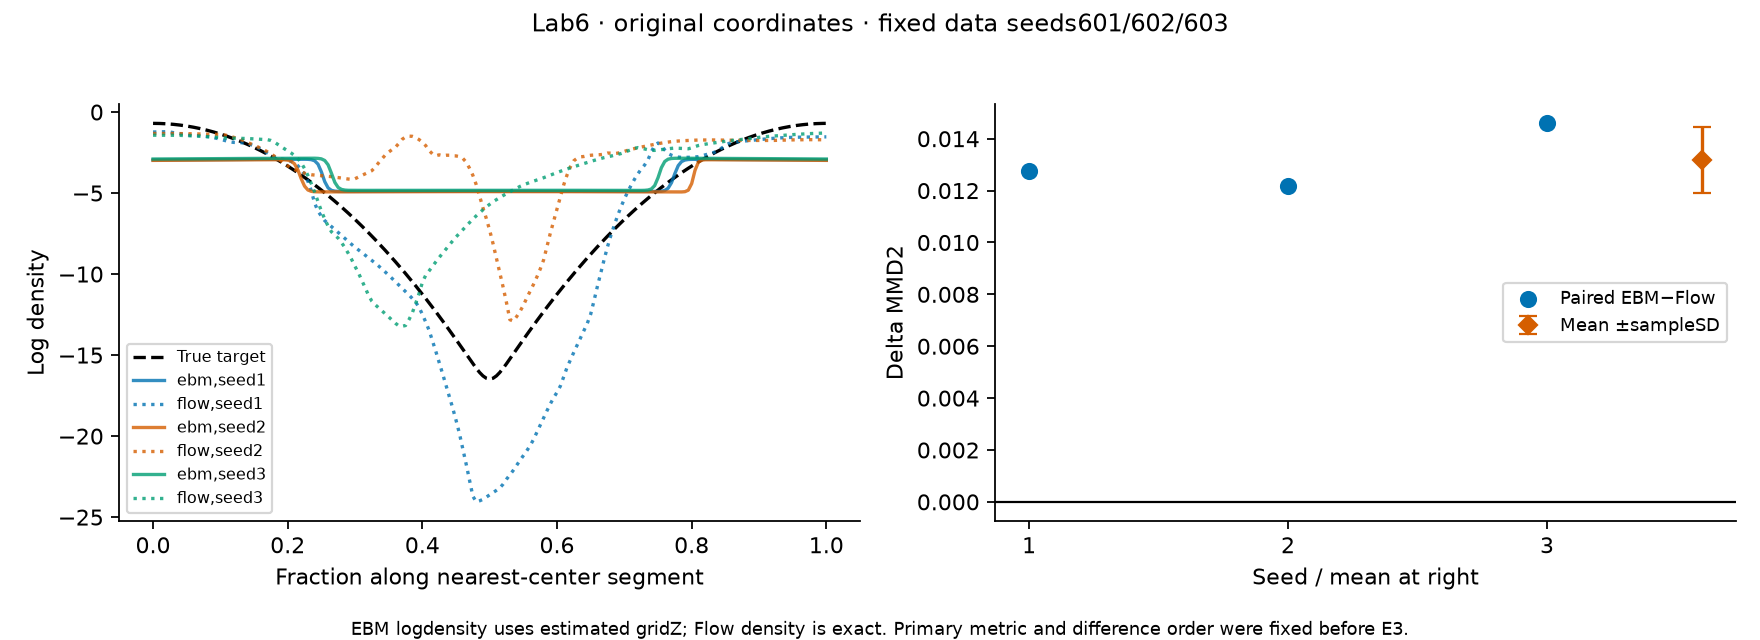
\includegraphics[width=\linewidth,height=.42\textheight,keepaspectratio]{figures/bridgefig.png}
\caption{Логарифмы плотности вдоль отрезка и три парные разности.}\label{fig:bridgefig}
\end{figure}

На seed 2 и 3 Flow переоценивает плотность середины примерно в 9718 и 48 549 раз, но на seed 1 она ниже истинной, отношение 0.000789. Поэтому выраженный мост не наблюдается одинаково во всех seed. Гауссовы компоненты имеют ненулевую плотность на всей плоскости: это не пример строго разорванного носителя. EBM тоже оставляет слишком много плотности в промежутке. Эти данные не доказывают единственный топологический механизм различия.

\section{Ответы на контрфактические вопросы}
\subsection*{Вопрос 1. Малый шаг при фиксированном K}
Два наименьших шага дали $D_K=0.892554$ и 1.728647. При фиксированном $K=50$ суммарный дрейф уменьшается с $\eta$, шумовой масштаб --- как $\sqrt{K\eta}$. Цепь остаётся возле старта; малый шаг не гарантирует близость короткой выборки к цели.
\subsection*{Вопрос 2. Максимальный шаг}
При $\eta=0.5$ квадратичная цепь дала 1.334314 против теоретических 1.333333, ошибка 0.0735\%. Выученная EBM устойчива, но Cov=0 и MMD$^2=0.203648$. Уже при минимальном шаге Cov=0, MMD$^2=0.052331$. На этой сетке первым выявлено плохое качество при сохранении численной устойчивости; порядок отказа Cov и MMD на более мелкой сетке неизвестен. Квадратичная формула не предсказывает покрытие нелинейной энергии.
\subsection*{Вопрос 3. Несогласованный шум}
При $\eta=0.5$, $\sigma=0.2$ эффективная температура $\sigma^2/(2\eta)=0.04$. Непрерывный квадратичный процесс имел бы дисперсию 0.04, дискретная рекурсия --- $0.04/(1-0.25)=0.053333$; измерено 0.053460. Цепь приближается к гауссовому стационарному закону дискретной рекурсии, который отличается от непрерывного температурного предела.
\subsection*{Вопрос 4. NLL и качество примеров}
При $K_f=8$ val NLL=1.134677, MMD$^2=0.000096807$; при 16 --- 1.139712 и 0.000074321. Ранги метрик расходятся. Однако разница MMD$^2=0.000022486$ меньше шума 0.000035877 для two blobs: надёжное преимущество генерации по этой паре не установлено. NLL оценивает плотность на данных, MMD --- близость генерируемого распределения.
\subsection*{Вопрос 5. Низкая энергия данных и промежуток}
Три логарифма для каждого seed приведены в таблице середины: например seed 2 даёт цель $-16.480539$, Flow $-7.298760$, EBM $-4.910132$. Низкая энергия данных сама по себе не ограничивает энергию промежутка, $Z$ или покрытие короткой цепи. Для EBM это только сеточная оценка на $\Omega$, для Flow --- точная плотность. Высота наблюдаемого моста зависит от оптимизации, глубины и базового распределения.

\noindent\textbf{Заключение.} Flow дал более качественные примеры на трудной цели в трёх seed. Корректная дисперсия и численная устойчивость Ланжевена не обеспечили смешивания и покрытия. Точное правдоподобие, обратимость и качество генерации требуют отдельных проверок.
\clearpage
\renewcommand{\refname}{Список использованных источников}
\begin{thebibliography}{9}
\addcontentsline{toc}{section}{Список использованных источников}
\bibitem{teacher} Лабораторная работа 6. Deep Energy-Based Models и Normalizing Flows. Density estimation, sampling, invertibility и ограничения представления распределений. Курс «Нейронные сети». Методические указания, 2026.
\end{thebibliography}
\clearpage
\section*{Приложение. Идентификация запусков}
\addcontentsline{toc}{section}{Приложение. Идентификация запусков}
\begingroup\small\setstretch{1.05}
\begin{longtable}{@{}l>{\raggedright\arraybackslash}p{3.5cm}p{10.8cm}@{}}
\caption{Полные RUN\_ID источников результатов.}\\
\toprule Код & Условие & RUN\_ID \\ \midrule \endhead
\hypertarget{R01}{R01} & E1 eta0.005 & {\fontsize{8.8}{11}\selectfont\texttt{134cc1ada1520a7482e7-d460ecfd9b1642fc9e2cf5b3c6f6d7ba}} \\
\hypertarget{R02}{R02} & E1 eta0.02 & {\fontsize{8.8}{11}\selectfont\texttt{9566292dba4841aae029-5961859ab47d43d5bd13594a7378baa4}} \\
\hypertarget{R03}{R03} & E1 eta0.08 & {\fontsize{8.8}{11}\selectfont\texttt{a2aa71727b0df9797290-ab2f5729578d4848953a9728cba469e8}} \\
\hypertarget{R04}{R04} & E1 eta0.5 & {\fontsize{8.8}{11}\selectfont\texttt{181a984d49ebf969ffe9-a4f272342fd9498899f4988990687960}} \\
\hypertarget{R05}{R05} & quadratic eta0.005 sigma0.1 & {\fontsize{8.8}{11}\selectfont\texttt{b213bcac0e2c91088c56-05aa515193a740399efe5090b54b6acf}} \\
\hypertarget{R06}{R06} & quadratic eta0.02 sigma0.2 & {\fontsize{8.8}{11}\selectfont\texttt{89b0840f07a02274e848-80015496fb1545b683f306136c51e56b}} \\
\hypertarget{R07}{R07} & quadratic eta0.08 sigma0.4 & {\fontsize{8.8}{11}\selectfont\texttt{c6d24fa02369d53d3666-6a24b1ac690245f39e4665397006782e}} \\
\hypertarget{R08}{R08} & quadratic eta0.5 sigma1.0 & {\fontsize{8.8}{11}\selectfont\texttt{e582a8a8c18deb14213c-a89bcdd573234772991b59efd1b4f2a3}} \\
\hypertarget{R09}{R09} & quadratic eta0.5 sigma0.2 & {\fontsize{8.8}{11}\selectfont\texttt{4a189c7de430dae3185e-c1f0345d63354e0781a36957c9b4cef4}} \\
\hypertarget{R10}{R10} & E2 depth2 & {\fontsize{8.8}{11}\selectfont\texttt{3e2187dd37b36a2bd1f4-234f10ef43c849029d91fc8cca2cf506}} \\
\hypertarget{R11}{R11} & E2 depth4 & {\fontsize{8.8}{11}\selectfont\texttt{cd7ee9b6a143040ac788-c7a3d8f7e6614b93a28ed0155caacf53}} \\
\hypertarget{R12}{R12} & E2 depth8 & {\fontsize{8.8}{11}\selectfont\texttt{a0314c5c3d42f5040040-6e051e63939e4c07846ff27ff10ff079}} \\
\hypertarget{R13}{R13} & E2 depth16 & {\fontsize{8.8}{11}\selectfont\texttt{6f7020df7a993543ca96-e9094c92df4a4acdb304487a46618133}} \\
\hypertarget{R14}{R14} & E3 ebm s1 & {\fontsize{8.8}{11}\selectfont\texttt{d20b01c7307c0257f2dd-15fc31e7e1964437b127450ffaac2fe0}} \\
\hypertarget{R15}{R15} & E3 flow s1 & {\fontsize{8.8}{11}\selectfont\texttt{cbfee41a37a5abc05267-03ff7991347b4adcb139e792bac0563e}} \\
\hypertarget{R16}{R16} & E3 ebm s2 & {\fontsize{8.8}{11}\selectfont\texttt{5146ebd52e80abca688c-8b1c99ce0b90452a8a5e9c185a9f3181}} \\
\hypertarget{R17}{R17} & E3 flow s2 & {\fontsize{8.8}{11}\selectfont\texttt{bab2188b75245e2f8cc6-eb1fc37eee9946628b3aa16785a17233}} \\
\hypertarget{R18}{R18} & E3 ebm s3 & {\fontsize{8.8}{11}\selectfont\texttt{a8da75f7a516997e4e82-8ccd9a201e074f289e6c29682a2d5a43}} \\
\hypertarget{R19}{R19} & E3 flow s3 & {\fontsize{8.8}{11}\selectfont\texttt{2a9a084eb89b7f2d68d6-5b4d9d6c2aa5417aa7f56898bf06b98e}} \\
\hypertarget{R20}{R20} & E1 EBM training & {\fontsize{8.8}{11}\selectfont\texttt{90803714ee7813d313f0-7741207547b7491dabeba08a2be0959d}} \\
\bottomrule\end{longtable}\endgroup
